\documentclass[border=4pt]{standalone}
\usepackage{tikz}
\usetikzlibrary{arrows.meta,calc,positioning,shapes.geometric}
\begin{document}
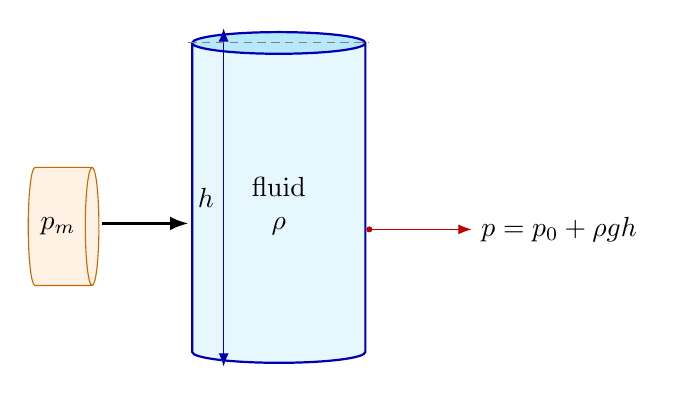
\begin{tikzpicture}[
  >=Latex,
  vessel/.style={cylinder,shape border rotate=90,shape aspect=.3,draw=blue!70!black,
    thick,minimum width=22mm,minimum height=42mm,outer sep=1.4pt,
    cylinder uses custom fill,cylinder body fill=cyan!10,cylinder end fill=cyan!28,
    align=center},
  sensor/.style={cylinder,shape aspect=.38,draw=orange!80!black,fill=orange!10,
    minimum width=15mm,minimum height=8mm,outer sep=1pt}
]
  \node[vessel] (tank) {fluid\\$\rho$};
  \node[sensor,anchor=mid east] (gauge)
    at ($(tank.mid west)+(-11mm,0)$) {$p_m$};

  \draw[-Latex,thick] (gauge.mid east) -- (tank.mid west);
  \draw[-Latex,red!75!black] (tank.base east) -- ++(13mm,0)
    node[right,black] {$p=p_0+\rho gh$};
  \draw[<->,blue!70!black]
    ($(tank.bottom)+(-7mm,0)$) -- node[left,black] {$h$}
    ($(tank.top)+(-7mm,0)$);
  \draw[densely dashed,gray] (tank.before top) -- (tank.after top);
  \fill[red!75!black] (tank.base east) circle (1.1pt);
\end{tikzpicture}
\end{document}
